\documentclass[11pt]{article}
\usepackage[utf8]{inputenc}
\usepackage[english]{babel}
\usepackage{amsfonts, amsmath, amssymb, amsthm}
\usepackage[none]{hyphenat}
\usepackage{fancyhdr}
\usepackage{graphicx}
\usepackage{float}
\usepackage{url}
\def\UrlBreaks{\do\/\do-}
\usepackage{breakurl}
\usepackage[breaklinks]{hyperref}
\usepackage[nottoc, notlot, notlof]{tocbibind}
\usepackage{algpseudocode}
\usepackage{mathtools}

\DeclarePairedDelimiter\floor{\lfloor}{\rfloor}

\graphicspath{{./}}

\theoremstyle{definition}
\newtheorem{definition}{Definition}[section]
\newtheorem{theorem}{Theorem}[section]
\newtheorem{claim}{Claim}[section]

\pagestyle{fancy}
\fancyhead{}
\fancyfoot{}
\fancyhead[L]{\slshape \MakeUppercase{Numerical Methods 1}}
\fancyhead[R]{\slshape \MakeUppercase{\today}}
\fancyfoot[C]{\thepage}
\fancyfoot[R]{\slshape \MakeUppercase{Elie Saad}}
\renewcommand{\headrulewidth}{0pt}

\begin{document}

\begin{titlepage}
\begin{center}
\vspace*{1cm}
\Large{\textbf{\MakeUppercase{Warsaw University of Technology}}}\\[3mm]
\huge{\textbf{Neural Networks}}\\[3mm]
\Large{\textbf{Faculty of Mathematics and Information Science}}\\
\vfill
\line(1,0){400}\\[1mm]
\huge{\textbf{Project 3}}\\[3mm]
\Large{\textbf{- Paper -}}\\[1mm]
\line(1,0){400}\\
\vfill
By \textbf{Elie SAAD}\\
\Large{\textbf{\today}}\\
\end{center}
\end{titlepage}

\tableofcontents
\thispagestyle{empty}
\clearpage

\section{Problem Statement}
A program which performs classification task with Multilayer Perceptron (MLP) network. The
program is trained with BACKPROPAGATION method or one of its extensions / modifications.

\section{Description}
We are to select two datasets from the UCI ML repository and come up with a program to perform training and testing on them.

\section{Datasets}
We have decided to choose two datasets:
\begin{itemize}
\item The Iris Data Set: which consists of four attributes and three classes.
\item The Adult Data Set: which consists of fourteen attributes and 2 classes.
\end{itemize}

\section{Proposed Solution}

\subsection{Preprocessing}
We took both datasets and applied the one hot encoding algorithm on both of their output vectors, meaning for the Iris dataset we have the three following vectors representing the three classes included in the dataset
\begin{itemize}
\item Iris Setosa which has an encoding vector of $\begin{pmatrix}1\\0\\0\end{pmatrix}$
\item Iris Versicolour which has an encoding vector of $\begin{pmatrix}0\\1\\0\end{pmatrix}$
\item Iris Virginica which has an encoding vector of $\begin{pmatrix}0\\0\\1\end{pmatrix}$
\end{itemize}
as for the Adults dataset, the following two vectors represent the two classes included in that dataset
\begin{itemize}
\item $>50K$ which has an encoding vector of $\begin{pmatrix}1\\0\end{pmatrix}$.
\item $\leq 50K$ which has an encoding vector of $\begin{pmatrix}0\\1\end{pmatrix}$.
\end{itemize}
We also proceeded to enumerate the various attributes that are not continuous from the Adults dataset i.e. Race, Sex, etc...

\subsection{Training}
We have given the user the full ability to pick and choose their preferred hidden layer combination. Every element in the $layers\_size$ vector represent the number of neurons, whereas the modulus of the $layers\_size$ vector represents the number of hidden layers.\\\\
The user can then select whichever dataset they desire to train the model on. Now let us briefly review the softmax and cross entropy functions, which are respectively the most commonly used activation and loss functions for creating a neural network for multi-class classification.\\\\
From the architecture of our neural network, we can see that we have three or two nodes in the output layer. We have several options for the activation function at the output layer. One option is to use sigmoid function.\\\\
However, there is a more convenient activation function in the form of softmax that takes a vector as input and produces another vector of the same length as output. Since our output contains three nodes, we can consider the output from each node as one element of the input vector. The output will be a length of the same vector where the values of all the elements sum to 1. Mathematically, the softmax function can be represented as
$$
y_i(z_i)=\frac{e^{z_i}}{\sum^k_{k=1}e^{z_i}}
$$ 
The softmax function simply divides the exponent of each input element by the sum of exponents of all the input elements. Let's take a look at a simple example of this\\\\
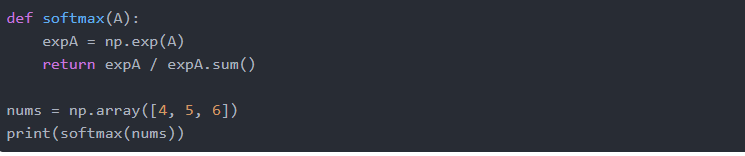
\includegraphics[scale=1]{image1.PNG}\\
In the script above we create a softmax function that takes a single vector as input, takes exponents of all the elements in the vector and then divides the resulting numbers individually by the sum of exponents of all the numbers in the input vector.\\\\
You can see that the input vector contains elements 4, 5 and 6. In the output, you will see three numbers squashed between 0 and 1 where the sum of the numbers will be equal to 1. The output looks likes this\\\\
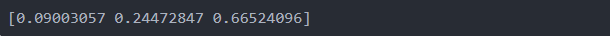
\includegraphics[scale=1]{image2.PNG}\\
Softmax activation function has two major advantages over the other activation functions, particular for multi-class classification problems: The first advantage is that softmax function takes a vector as input and the second advantage is that it produces an output between 0 and 1. Remember, in our dataset, we have one-hot encoded output labels which mean that our output will have values between 0 and 1. However, the output of the feedforward process can be greater than 1, therefore softmax function is the ideal choice at the output layer since it squashes the output between 0 and 1.\\\\
With softmax activation function at the output layer, mean squared error cost function can be used for optimizing the cost as we did in the previous articles. However, for the softmax function, a more convenient cost function exists which is called cross-entropy.\\\\
Mathematically, the cross-entropy function looks likes this
$$
H(y,\hat{y})=-\sum_iy_i\log\hat{y}_i
$$
The cross-entropy is simply the sum of the products of all the actual probabilities with the negative log of the predicted probabilities. For multi-class classification problems, the cross-entropy function is known to outperform the gradient decent function.\\\\
Now that we have sufficient knowledge to create a neural network that solves multi-class classification problems. In what follows we will show how the model will work.\\\\

\subsubsection{Feed Froward}
The feed forward phase will be be divided into two phases, the phase of the hidden layers where they use the sigmoid function as an activation function, and the output layer where it uses the softmax activation function to make its prediction vectors.\\\\
In the first phase, we will see how to calculate output from the hidden layer. For each input record, we have either four or fourteen features. To calculate the output values for each node in the hidden layer, we have to multiply the input with the corresponding weights of the hidden layer node for which we are calculating the value. Notice, we are also adding a bias term here. We then pass the dot product through sigmoid activation function to get the final value. \\\\
For instance to calculate the final value for the first node in the hidden layer, which is denoted by "ah1", you need to perform the following calculation\\
$$
zh1=\sum_ixiwi+b
$$
$$
ah1=\frac{1}{1+e^{-zh1}}
$$
This is the resulting value for the top-most node in the hidden layer. In the same way, we calculate te values of all the nodes in the hidden layer.\\\\
To calculate the values for the output layer, the values in the hidden layer nodes are treated as inputs. Therefore, to calculate the output, multiply the values of the hidden layer nodes with their corresponding weights and pass the result through an activation function, which will be softmax in this case.\\\\
This operation can be mathematically expressed by the following equation
$$
zoi=\sum_jahjwj
$$
Here $zoi$ will form the vector that we will use as input to the sigmoid function. Lets name this vector "$zo$". Let $j=3$ for instance, then $zo$ is denoted as\\\\
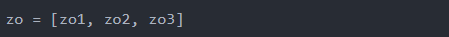
\includegraphics[scale=1]{image3.PNG}\\
Now to find the output value a01, we can use softmax function as follows
$$
ao1(zo)=\frac{e^{zo1}}{\sum^k_{k=1}e^{zok}}
$$
Here "$a01$" is the output for the top-most node in the output layer. In the same way, we use the softmax function to calculate the values for all the $aoi$'s.

\subsubsection{Back-Propagation}
The basic idea behind back-propagation remains the same. We have to define a cost function and then optimize that cost function by updating the weights such that the cost is minimized. However, we will use cross-entropy function to calculate the error.\\\\
To find the minima of a function, we can use the gradient decent algorithm. The gradient decent algorithm can be mathematically represented as follows
$$
repeat\textrm{ }until\textrm{ }convergence:\{w_j:=w_j-\alpha \frac{\partial}{\partial w_j}J(w_0,w_1,...,w_n)\}
$$
The details regarding how gradient decent function minimizes the cost have already been discussed in the previous article. Here we will jus see the mathematical operations that we need to perform.\\\\
Our cost function is
$$
H(y,\hat{y})=-\sum_iy_i\log\hat{y}_i
$$
In our neural network, we have an output vector where each element of the vector corresponds to output from one node in the output layer. The output vector is calculated using the softmax function. If "ao" is the vector of the predicted outputs from all output nodes and "y" is the vector of the actual outputs of the corresponding nodes in the output vector, we have to basically minimize this function
$$
cost(y,ao)=-\sum_iy_i\log ao_i
$$
In the first phase, we need to update weights  of the output layer nodes.\\\\
We know from class that to minimize the cost function, we have to update weight values such that the cost decreases. To do so, we need to take the derivative of the cost function with respect to each weight. Mathematically we can represent it as
$$
\frac{dcost}{dwo}=\frac{dcost}{dao}*\frac{dao}{dzo}*\frac{dzo}{dwo}
$$
Here "wo" refers to the weights in the output layer.\\\\
The first part of the equation can be represented as
$$
\frac{dcost}{dao}*\frac{dao}{dzo}
$$
The derivative of the above equation is
$$
\frac{dcost}{dao}*\frac{dao}{dzo}=ao-y
$$
Where "ao" is predicted output while "y" is the actual output.\\\\
Finally, we need to find "dzo" with respect to "dwo" from the first equation. The derivative is simply the outputs coming from the hidden layer as shown below
$$
\frac{dzo}{dwo}=ah
$$
To find new weight values, the values returned by the first equation can be simply multiplied with the learning rate and subtracted from the current weight values.\\\\
We also need to update the bias "bo" for the output layer. We need to differentiate our cost function with respect to bias to get new bias value as shown below
\begin{equation}
\frac{dcost}{dbo}=\frac{dcost}{dao}*\frac{dao}{dzo}*\frac{dzo}{dbo}
\end{equation}
The first part of the Equation 1 has already been calculated in the previous equation. Here we only need to update "dzo" with respect to "bo" which is simply 1. So
\begin{equation}
\frac{dcost}{dbo}=ao-y
\end{equation}
To find new bias values for output layer, the values returned by Equation 2 can be simply multiplied with the learning rate and subtracted from the current bias value.\\\\
In the second phase, we will back-propagate our error to the previous layer and find the new weight values for hidden layer weights of the hidden layer.\\\\
Let's collectively denote hidden layer weights as "wh". We basically have to differentiate the cost function with respect to "wh".\\\\
Mathematically we can use chain rule of differentiation to represent it as
\begin{equation}
\frac{dcost}{dwh}=\frac{dcost}{dah}*\frac{dah}{dzh}*\frac{dzh}{dwh}
\end{equation}
Here again, we will break Equation 3 into individual terms.\\\\
The first term "dcost" can be differentiated with respect to "dah" using the chain rule of differentiation as follows
\begin{equation}
\frac{dcost}{dao}*\frac{dao}{dzo}=\frac{dcost}{dzo}==ao-y
\end{equation}
Now we need to find dzo/dah from Equation 4, which is equal to the weights of the output layer as shown below
\begin{equation}
\frac{dzo}{dah}=wo
\end{equation}
Now we can find the value of dcost/dah by replacing the values from Equations 4 and 5 in Equation 3.\\\\
Coming back to Equation 2, we have yet to find dah/dzh and dzh/dwh.\\\\
The first term dah/dzh can be calculated as
\begin{equation}
\frac{dah}{dzh}=sigmoid(zh)*(1-sigmoid(zh))
\end{equation}
And finally, dzh/dwh is simply the input values
\begin{equation}
\frac{dzh}{dwh}=input\textrm{ }features
\end{equation}
If we replace the values from Equations 3, 6 and 7 in Equation 2, we can get the updated matrix for the hidden layer weights. To find new weight values for the hidden layer weights "wh", the values returned by Equation 3 can be simply multiplied with the learning rate and subtracted from the current hidden layer weight values.\\\\
Similarly, the derivative of the cost function with respect to hidden layer bias "bh" can simply be calculated as
\begin{equation}
\frac{dcost}{dbh}=\frac{dcost}{dah}*\frac{dah}{dzh}*\frac{dzh}{dbh}
\end{equation}
Which is simply equal to
\begin{equation}
\frac{dcost}{dbh}=\frac{dcost}{dah}\frac{dah}{dzh}
\end{equation}
because
\begin{equation}
\frac{dzh}{dbh}=1
\end{equation}
To find new bias values for the hidden layer, the values returned by Equation 10 can be simply multiplied with the learning rate and subtracted from the current hidden layer bias values and that is it for the back-propagation.

\section{Testing}
In the following three images we made three networks which have 10x10, 5x5, and 20x20x20 hidden layers. The following are the results of our tests\\\\
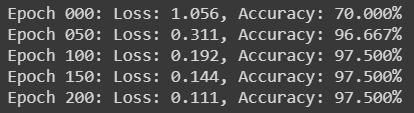
\includegraphics[scale=1]{image4.PNG}\\\\
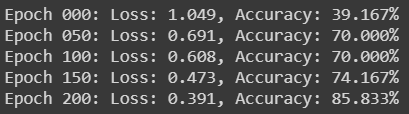
\includegraphics[scale=1]{image5.PNG}\\\\
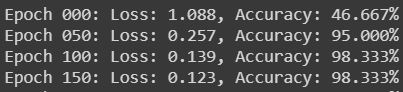
\includegraphics[scale=1]{image6.PNG}
\end{document}